\documentclass[11pt]{article}

\usepackage[margin=1in]{geometry}
\usepackage{amsmath,amssymb,amsthm}
\usepackage{graphicx}
\usepackage[hidelinks]{hyperref}

\newtheorem*{theorem}{Theorem}

\newcommand{\ellTwo}{\ell_2}

\begin{document}

\begin{center}
{\Large Literature status: superreflexive \(\Delta\)-point subcases of Question 7.7}

\medskip
{\small Run \texttt{fa\_banach\_001}; source arXiv:2301.04433}
\end{center}

\section*{Packet Status}

This packet records a literature-already-answered partial subcase, not an
original construction from the run.  The supporting paper explicitly cites
Martin--Perreau--Rueda Zoca Question 7.7 and constructs a superreflexive
example with strong \(\Delta\)-type points.  The packet does not answer the
Daugavet or super Daugavet parts of the source question.

\section*{Source Question}

The source is Miguel Martin, Yoel Perreau, and Abraham Rueda Zoca,
\emph{Diametral notions for elements of the unit ball of a Banach space},
arXiv:2301.04433.  Question 7.7 asks for isomorphic restrictions on Banach
spaces containing \(\Delta\)-points or the other diametral notions, and then
asks in particular whether a reflexive, or even super-reflexive, Banach space
can contain \(\Delta\)-, super \(\Delta\)-, ccs \(\Delta\)-, Daugavet, or
super Daugavet points.

\begin{center}

\includegraphics[width=\textwidth]{figures/open_problem_crop.png}
\end{center}

\section*{Supporting Literature}

The supporting paper is Trond A. Abrahamsen, Ramon J. Aliaga, Vegard Lima,
Andre Martiny, Yoel Perreau, Antonin Prochazka, and Triinu Veeorg,
\emph{Delta-points and their implications for the geometry of Banach spaces},
arXiv:2303.00511.  Its introduction states that Question 7.7 of
Martin--Perreau--Rueda Zoca asks whether finite-dimensional nonexistence of
\(\Delta\)-points also holds for superreflexive spaces, and says this is
answered negatively in Section 3.

The key supporting theorem is Theorem 3.1.

\begin{center}
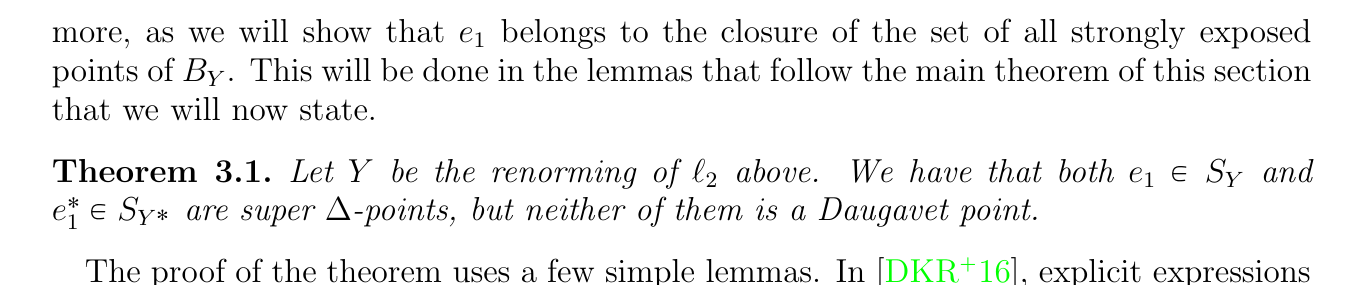
\includegraphics[width=\textwidth]{figures/supporting_theorem_3_1_crop.png}
\end{center}

The same section then records that the points are actually ccw
\(\Delta\)-points.

\begin{center}
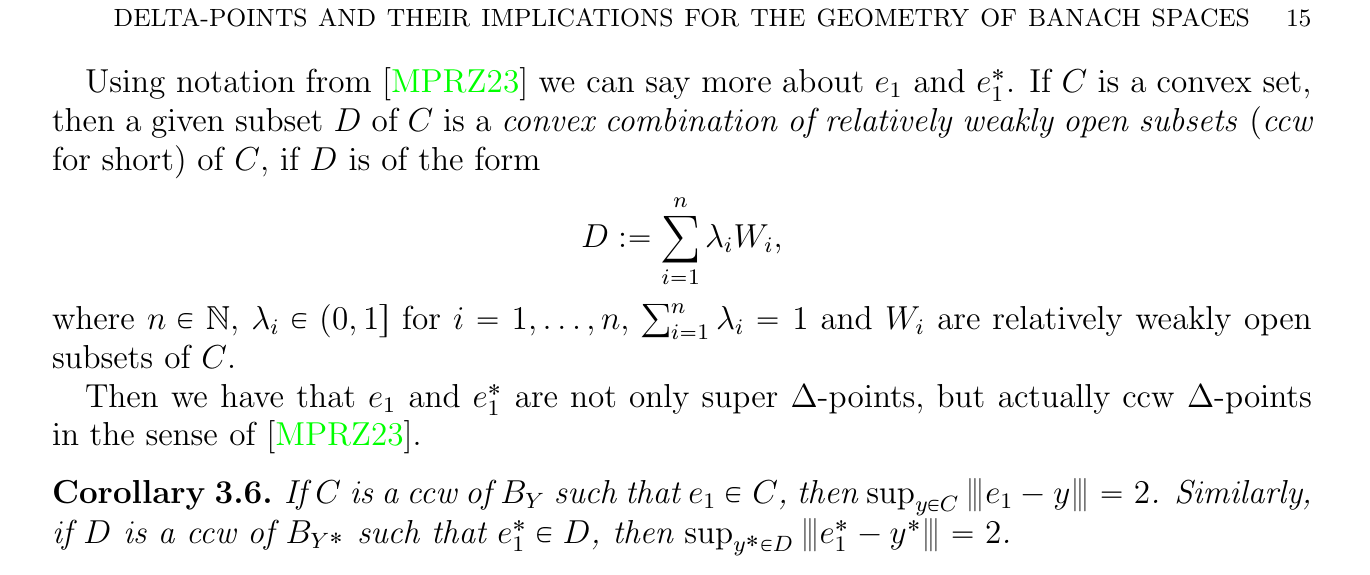
\includegraphics[width=\textwidth]{figures/supporting_ccw_corollary_crop.png}
\end{center}

\section*{Idea of the Proof}

The source question asks whether even superreflexive spaces can support these
diametral point notions.  The supporting paper builds an equivalent norm on
\(\ellTwo\).  Equivalent renorming preserves the isomorphic property of
superreflexivity.  The supporting theorem then marks \(e_1\) as a super
\(\Delta\)-point, and the following corollary upgrades it to ccw
\(\Delta\).  Since every slice is a relatively weakly open subset, ccw
\(\Delta\) implies ccs \(\Delta\); and super \(\Delta\) implies ordinary
\(\Delta\).

\section*{Formal Statement}

\begin{theorem}
There is a superreflexive Banach space containing a point that is
simultaneously a \(\Delta\)-point, a super \(\Delta\)-point, and a ccs
\(\Delta\)-point.  Consequently, Question 7.7 of arXiv:2301.04433 has an
affirmative answer for these three diametral notions.
\end{theorem}

\begin{proof}
Let \(Y\) be the equivalent renorming of \(\ellTwo\) constructed in Section 3
of arXiv:2303.00511.  Since \(Y\) is linearly isomorphic to Hilbert space
\(\ellTwo\), it is superreflexive.

Theorem 3.1 of arXiv:2303.00511 states that \(e_1\in S_Y\) is a super
\(\Delta\)-point.  In particular, \(e_1\) is a \(\Delta\)-point, because
slices containing \(e_1\) are special cases of relatively weakly open subsets
of \(B_Y\) containing \(e_1\).

Corollary 3.6 of the same paper states that \(e_1\) is a ccw
\(\Delta\)-point: for every convex combination of relatively weakly open
subsets \(C\) of \(B_Y\) with \(e_1\in C\), one has
\[
  \sup_{y\in C}\vert\!\vert\!\vert e_1-y\vert\!\vert\!\vert=2.
\]
Every convex combination of slices is a convex combination of relatively
weakly open subsets.  Hence \(e_1\) is also a ccs \(\Delta\)-point.

Thus the superreflexive space \(Y\) gives affirmative examples for the
\(\Delta\), super \(\Delta\), and ccs \(\Delta\) parts of Question 7.7.
\end{proof}

\section*{Limitations}

This is only a partial subcase of Question 7.7.  It does not answer whether a
reflexive or superreflexive Banach space can contain a Daugavet point or a
super Daugavet point.  Indeed, Theorem 3.1 of the supporting paper explicitly
states that the points \(e_1\in S_Y\) and \(e_1^*\in S_{Y^*}\) are not
Daugavet points.

\section*{Literature And Duplicate Check}

The run lightweight indexes were searched for arXiv:2301.04433, diametral
notions, \(\Delta\)-points, Daugavet points, ccs \(\Delta\)-points, and
superreflexive/reflexive keywords.  No existing packet, attempt, or proof-gap
entry covered Question 7.7.  The only nearby registry hit for arXiv:2303.00511
was a different full packet concerning weak-star \(\Delta\)-points in duals of
subspaces with shrinking \(k\)-unconditional bases.

\section*{Human Review Recommendation}

Review as a literature-already-answered partial subcase.  The main checks are:
the identification of \(Y\) as a superreflexive renorming of \(\ellTwo\), the
implication ccw \(\Delta\Rightarrow\) ccs \(\Delta\), and the stated scope
exclusion for Daugavet and super Daugavet points.

\begin{thebibliography}{9}

\bibitem{MPRZ}
M. Martin, Y. Perreau, and A. Rueda Zoca,
\emph{Diametral notions for elements of the unit ball of a Banach space},
arXiv:2301.04433.

\bibitem{AALMPPV}
T. A. Abrahamsen, R. J. Aliaga, V. Lima, A. Martiny, Y. Perreau,
A. Prochazka, and T. Veeorg,
\emph{Delta-points and their implications for the geometry of Banach spaces},
arXiv:2303.00511.

\end{thebibliography}

\end{document}
